\documentclass[problem]{mcs}

\begin{pcomments}
  \pcomment{CP_coloring}
  \pcomment{first part appears as MQ_coloring_short}
\end{pcomments}

\pkeywords{
  coloring
  cycle
  chromatic_number
  subgraph
  K_4
  complete_graph
}

%%%%%%%%%%%%%%%%%%%%%%%%%%%%%%%%%%%%%%%%%%%%%%%%%%%%%%%%%%%%%%%%%%%%%
% Problem starts here
%%%%%%%%%%%%%%%%%%%%%%%%%%%%%%%%%%%%%%%%%%%%%%%%%%%%%%%%%%%%%%%%%%%%%

\begin{problem}

\begin{problemparts}

\problempart Determine a valid coloring of the graph shown in
Figure~\ref{fig:to_color} using as few colors as possible.  (Simply
write your proposed color for each vertex next to that vertex.  You
may use $R$ for red, $G$ for green, etc.)

\begin{figure}[h]
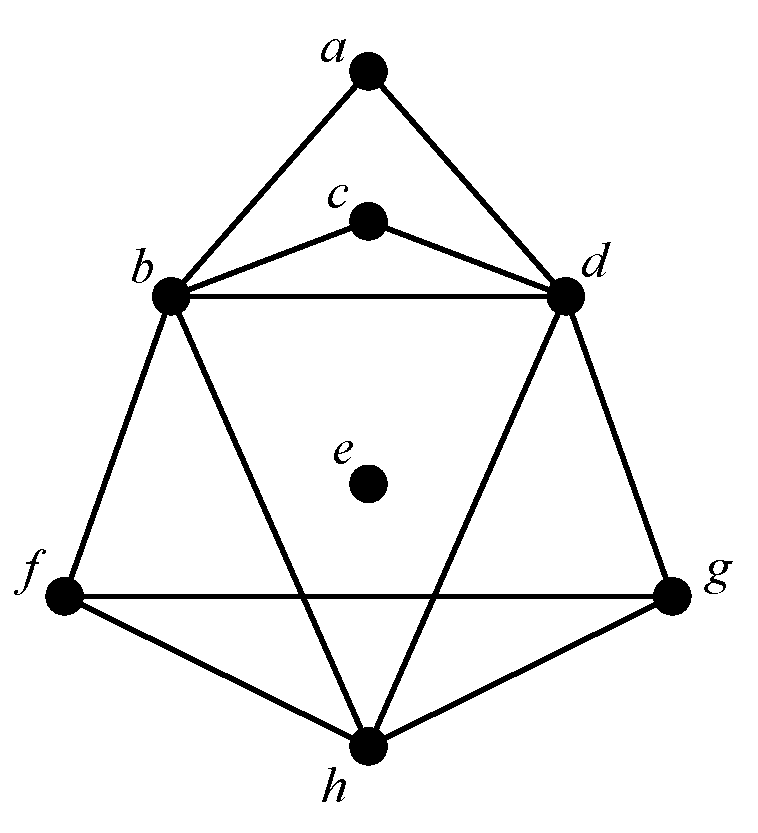
\includegraphics[width = 3in]{MQ_coloring}
\caption{\label{fig:to_color}}
\end{figure}

\examspace[1in]

\begin{solution}
There are odd-length cycles in the graph, so at least three colors
will be needed.  So assume that three colors are sufficient.  (If we
encounter a contradiction under this assumption, we will need to use
more colors.)  Start with the length-3 cycle $abda$.  All of its
vertices must be colored differently, so assign red to $a$, blue to
$b$, and green to $d$.  The length-3 cycle $bdhb$ now forces $h$ to be
colored red.  $f$ must now be colored green and $g$ must be colored
blue.  The coloring is valid so far.  $c$ is adjacent to a blue vertex
and a green vertex, and no others, it must be colored red.  Finally,
$e$ is not adjacent to any other vertices, so it can be assigned any
of the three colors.  Choosing red for $e$, the result is shown in
Figure~\ref{fig:colored}.  There is no pair of like-colored adjacent
vertices, so this coloring is valid.
\begin{figure}[h]
\graphic{MQ_coloring_sol}
\caption{A valid coloring.\label{fig:colored}}
\end{figure}
\end{solution}

\problempart
What is the chromatic number of the graph?

\examspace[1in]

\begin{solution}
Three.  As already discussed, fewer than three colors are
insufficient, and three colors can be used to create a valid coloring.
\end{solution}

\problempart Is it possible to increase the chromatic number of the
graph by adding just one edge?  If yes, state which new edge would do
the trick.  If no, explain why.

\examspace[2in]

\begin{solution}
Certainly.  There are a few possibilies.  For instance, adding
$\edge{a}{c}$ creates a subgraph isomorphic to $K_4$.  Since
$\chi(K_4)=4$, the resulting graph would have a chromatic number of at
least four.  (Exaclty four, in fact.)
\end{solution}

\problempart Is it possible to decrease the chromatic number of the
graph by removing just one edge?  If yes, state which edge could be
removed to do the trick.  If no, explain why.

\examspace[2in]

\begin{solution}
No.  No matter which edge is removed, the graph will still contain
odd-length cycles as subgraphs.  The chromatic number of the graph
would thus still be at least three.  (Exactly three, actually.)
\end{solution}

\end{problemparts}
\end{problem}

\endinput
